\documentclass[11pt]{wbzine}
%packages
\usepackage{lipsum}
\usepackage[utf8]{inputenc}
\usepackage[T1]{fontenc}
\usepackage[ngerman]{babel}
\usepackage{coelacanth}
\usepackage{pdfpages}
\usepackage{tocloft}
\renewcommand{\cftsecfont}{\mdseries}
\renewcommand{\cftsecpagefont}{\mdseries}
% needed for phf session form article
\usepackage{fourier-orns}
\usepackage{wasysym}
\newcommand{\monster}{\textxswup}
\newcommand{\torch}{\sun}
\newcommand{\lantern}{\CIRCLE}
%
\setlength{\leftmargini}{1em}
\begin{document}

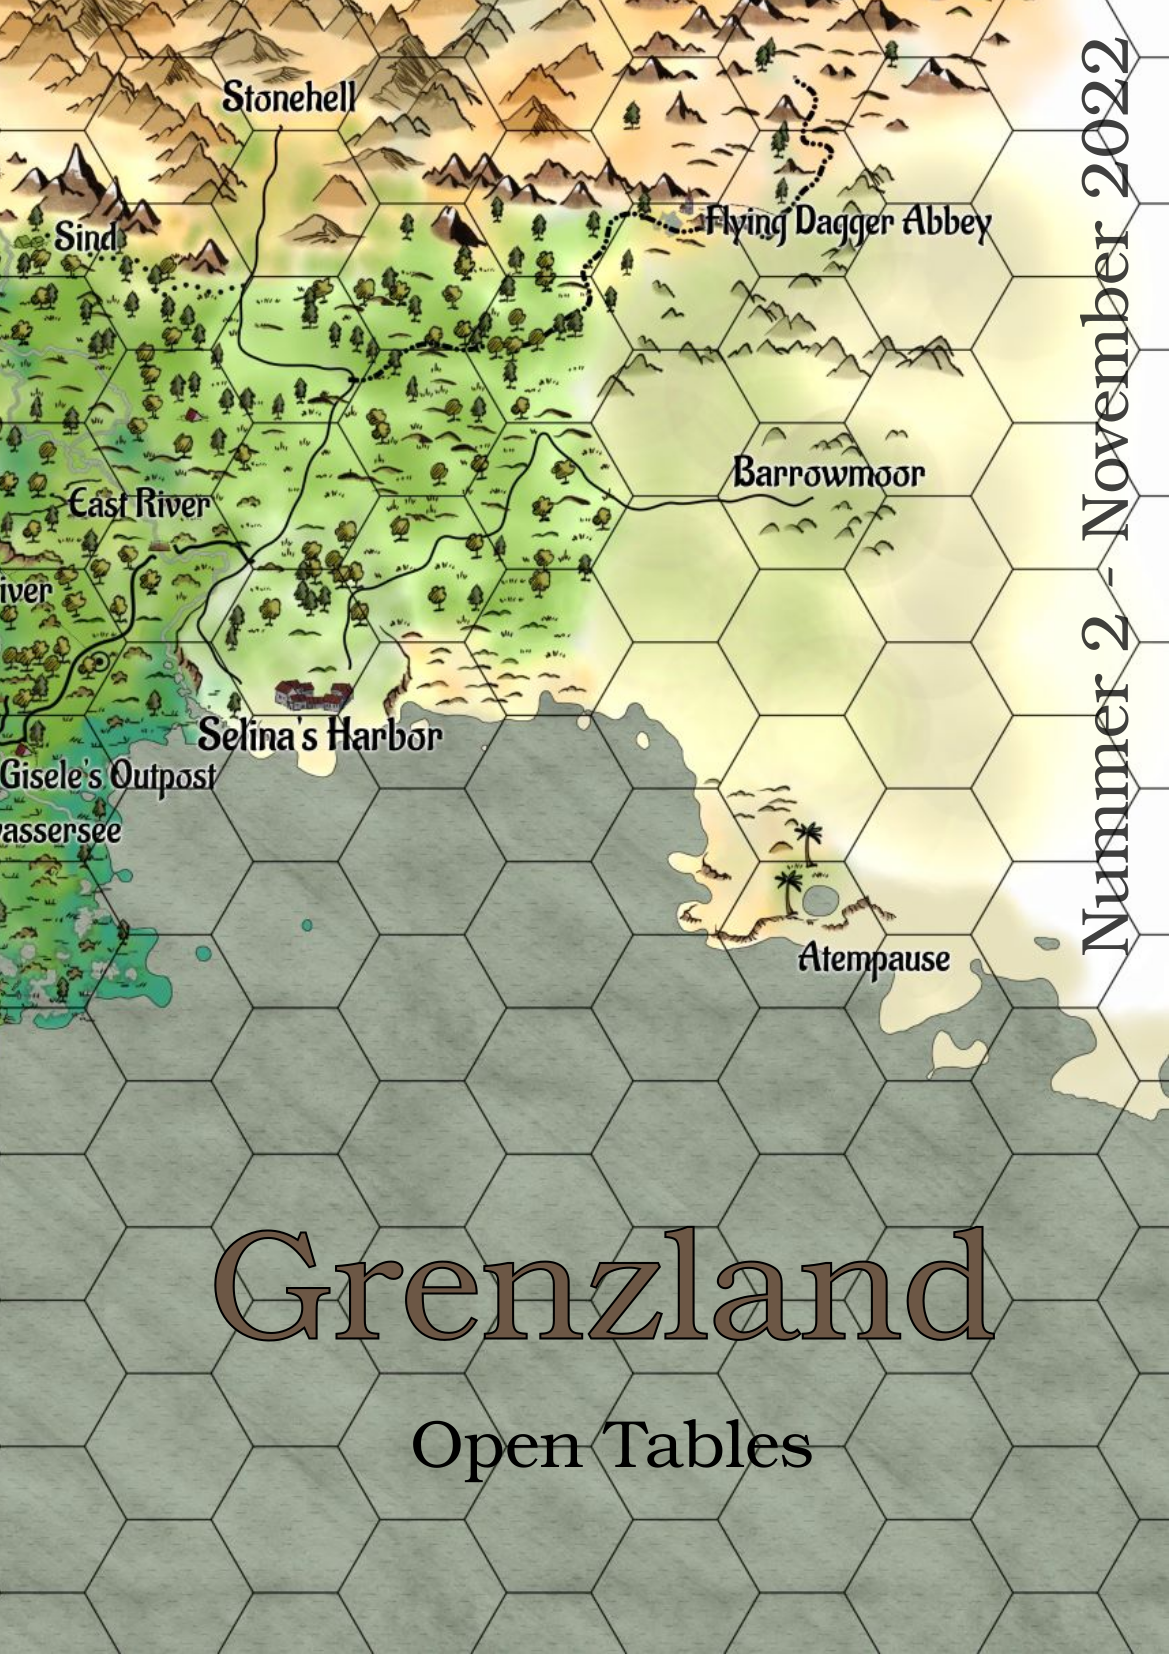
\includepdf{Frontcover.pdf}

\shipout\null
\addtocounter{page}{-1}

{\bfseries\fontsize{70}{55}
 \selectfont Grenzland \par}%
 \hrulefill
 Nummer 2, April 2023

\tableofcontents

\begin{multicols}{2}

\section{Vorwärts!}

Sören erzählt, wie er zur Gruppe stieß und neue Erfahrungen mit dem
    alten Konzept der Open Tables machte, und gibt uns auf diesem
    Weg eine hervorragende Einleitung.

Alex und Peter erklären, worum es sich bei den Open Tables handelt

Alex berichtet von den Exkursionen in die Steinhölle.

Peter berichet von den Abenteuern im Hügelgräberlabyrinth, erzählt
    wie er dem Spiel einen saisonmäßigen touch gegeben hat, und
    erklärt ein praktisches Tool, um während des Spielleitens den
    Überblick zu behalten.

    Olupo erzählt über seine \textit{Zisterne der Auferstehung}, und
    lässt uns sogar hinter die Kulissen schauen.



\by{lkh}

\section{Altes Konzept für Neue Welten}
Von einem offenen Tisch (Open Table) hatte ich schon gehört, aber bis
zu jenem schicksalhaften Abend im Juni 2022 hatte ich noch nie direkt
damit zu tun gehabt. (Denn auch wenn ich diesem Hobby schon seit mehr
als 25 Jahren fröne, war es Mitte der 90er auf dem platten Land noch
nicht weit her mit der Anzahl der Spielenden.) Und so kam es, dass ich
mir ziemlich spontan eine Figur ausgesucht und meine erste Runde bei Alex
gespielt habe. Zuerst war ich skeptisch ob ein zusammengewürfelter Haufen
von Menschen in der Kürze der Zeit überhaupt ein zufriedenstellendes
Spielerlebnis bieten würde, aber ich wurde eines besseren belehrt.

Die Kürze der Termine (zwei Stunden) sorgte dafür, dass die volle
Konzentration aller Menschen am (virtuellen) Tisch vorhanden war. Gerade
beim Onlinespiel habe ich die Erfahrung gemacht, dass weniger oft
mehr ist. Nicht nur sind zwei Stunden viel einfacher, auch unter der
Woche, einzuplanen, sondern es ist auch weniger anstrengend mit voller
Konzentration dabei zu sein.

Durch den offenen Tisch war es auch egal wer der anderen Spielenden (und
sogar der Spielleitung) am nöchsten Termin Zeit hatte. Ausschlaggebend
war nur, dass sich genügend Menschen fanden die Bock hatten zu
spielen. Nicht wenige Termine fanden mit nur ein paar Stunden Vorlauf
für die Planung statt, was mit einer festen Gruppe von Spielenden
ziemlich sicher an anderen Terminen gescheitert wäre.

Ein dreiviertel Jahr später habe ich mit den unterschiedlichsten
Menschen gespielt und einige Ausflüge in die Steinhölle, das
Hügelgräberlabyrinth und die Zisterne der Auferstehung hinter mir und
ich bin wieder dabei wenn es zeitlich passt. Auch bin ich mir sicher,
dass das "alte" Konzept des offenen Tisches sich sehr gut für die "neuen"
Welten des Onlinespiels eignet, da beider Stärken in meinen Augen sehr
gut ineinandergreifen.
\by{ff}

\section{Ein offener Tisch mit Mehrpersonenspielleitung}

Ein “offener Tisch” ist ein Organisationsform für Pen-\&-Paper-Rollenspiele.
Die Spielercharaktere befinden sich an einem “sicheren” Ort, meistens einer
zentralen Siedlung. Spielerinnen und Spieler können ihre Charaktere zu jedem
Spiel mitnehmen. Zu beachten ist nur, dass die Zeit genau gleich wie in der
Realität verstreicht: Wenn ein Charakter im Spiel eine Woche auf Reise ist,
oder sich erholen muss, dann steht der Charakter entsprechen lange nicht zur
Verfügung.

Die Spielerinnen und Spieler spielen in wechselnder Zusammensetzung. Wenn am
nächsten Termin ein Platz frei wird, kann eine andere Person mit ihrem eigenem
Charakter einspringen: die Gruppenmitglieder sind nicht fix und im Spiel
probieren wir das so zu handhaben, dass jeder Spielabend eine Expedition ist,
die wieder in einer sicheren Gegend endet, so dass es auch einigermassen
plausibel ist, wenn sich die Zusammensetzung der Gruppe ändert.

Viele der ``Montagsspiele'' auf dem Grenzland Server sind ein offener Tisch.
Ausserdem gibt es mehrere Spielleiterinnen und Spielleiter die jeweils für
eine eigene Gegend zuständig sind. Die Landkarte auf dem Cover zeigt die
gesamte Region dieser Kampagne. Alex leitet die Steinhölle (Stonehell) und die
Riesigen Riesen (die Region nördlich von Selina's Harbor, unserem Startdorf),
Peter leitet das Hügelgräberlabyrinth (Barrowmaze) und Frotz leitet die
Wurfmesserküste (The Flying Dagger Coast, die Region westlich von Selina's
Harbor). Alle verwenden den gleichen Pool an Spielercharakteren, das gleiche
Setting und (weitgehend) die gleichen Regeln.

Wir spielen aus Rücksicht auf Frühaufsteher und Familien normalerweise
Wochentags von 20:15 bis 22:00, deswegen muss alles recht zügig gehen. Da
bleibt wenig Zeit für Stimmungsspiel und Taschenlampenfallenlassen. Die
erfahrenen Spielerinnen und Spieler machen entsprechend etwas mehr Druck, da
sie genau wissen, dass wir nur wenig Zeit haben. Beispielsweise wird nicht
ausgespielt, wie in Selina's Harbor eingekauft wird und Spielercharaktere
machen nur selten absichtlich Dummheiten im Dungeon weil alle Früher oder
Später erfahren haben wie gefährlich so ein Dungeon ist. Nicht bis zur letzten
Sekunde zu warten um den Dungeon wieder zu verlassen gehört auch zum guten Ton,
schliesslich weiss niemand ob auf dem Weg nach draussen nicht doch noch ein
Monster auftaucht.

\textbf{Jeder ist herzlich eingeladen mitzuspielen!} Einfach dem Grenzland
Discord-Server beitreten und sich im Kanal \#montag melden!
\by{alex,~phf}


\section{Die Steinhölle (Stonehell Dungeon)}

\textbf{Referee}: Alex

\textbf{Zahlen}: siehe Beschreibung

    \textbf{Beschreibung}: Alex leitet den Stonehell Dungeon von
    \textit{Michael Curtis}. Das ist ein Dungeon in zwei Büchern
    über 10 Ebenen, jede Ebene besteht aus 4 Quadranten und jeder
    Quadrant hat etwa 40 Räume. Zudem gibt es an der Oberfläche noch
    zwei Quadranten mit einer alten Torhaus, ein paar Höhlen und
    kleinen Komplexen. Auf den ersten Blick sieht die Oberfläche
    sehr nach den “Caves of Chaos” (aus B2: Die Festung im
    Grenzland\footnote{Die Chaoshöhlen sind so manchem Grenzländer
    gut bekannt. Sie waren der Ausgangspunkt für die gleichnamige
    Grenzland-Kampagne, die diesem Zine, und unserem Discord-Server
    den Namen gaben (Anm. d. Red.)}) aus. Aktueller Stand: Die
    Spielerinnen und Spieler haben die beiden Quadranten der
    Oberfläche und drei Quadranten der ersten Ebene betreten.
    Bleiben noch 37 Quadranten zu erforschen.

    Bisher hat man Orks und Banditen bedroht, verprügelt und
    ausgeraubt; sich mit Ghulen angelegt; einen Bär, einen Puma und
    einen Riesengecko erschlagen, einen anderen Riesengecko
    regelmässig gefüttert; ist an Schlangengift und Spinnengift
    gestorben oder ist erstochen worden; hat Fallen entschärft,
    Diebe bezaubert, grünen Schleim gefunden, ist Stufe gestiegen,
    hat einen Hobgoblin Aussenposten übernommen und gesichert…

    Die aktuelle Spielerzahl ist etwas schwer zubestimmen, da die
    gleichen Spielercharaktere auf für Expeditionen ins
    Hügelgräberlabyrinth (Barrowmaze), an die Wurfmesserküste und in
    die Riesigen Riesen verwendet werden. Die Charaktere der
    inaktiven Spielerinnen und Spieler werden wieder freigegeben, so
    das sicher drei Spielerinnen und Spieler aus der Liste wieder
    verschwunden sind. Im Moment stehen zwanzig aktive Spielerinnen
    und Spieler mit mindestens einem Charakter auf der Liste. Hierzu
    muss man allerdings sagen, dass manche zwar “aktiv” sind, weil sie in
    den letzten Wochen mitgespielt haben, es für einige allerdings
    auch ihr erstes und einziges Mal war.
\by{alex,~phf}


\section{Das Hügelgräberlabyrinth (Barrowmaze)}

\textbf{Referee:} Peter

\textbf{Zahlen:} 30 Sessions (März 2022--April 2023),
insgesamt 16 Spieler,
3--5 Spieler regelmässig aktiv,
aktivster Spieler hat 19 Sessions,
aber 7 Spieler waren nur ein- oder zweimal dabei

\textbf{Beschreibung}: Peter leitet Barrowmaze von \textit{Greg Gillespie}.
Im Gegensatz zu den meisten Dungeons geht Barrowmaze nicht ``tiefer'' nach
unten sondern ``weiter'' nach Norden, Süden, und vor allem Osten. An der
Oberfläche sind Dutzende von Hügelgräbern und einige davon sind (mehr oder
weniger) mit den Katakomben des Barrowmaze verbunden. Ja, da hats viele
Untote. Auch Ungeziefer und Riesenfrösche und so weiter, aber eben auch
viele Untote. Und da die Regeln nach denen wir spielen keine Kleriker
vorsehen\dots{}

Peter hat das erste Barrowmaze Buch und keine der weiteren. Aber das ist
nicht wirklich ein Problem weil die Spieler bis jetzt in 30 Sessions noch
nicht einmal 20\% des Dungeons erforscht haben. Ausserdem hat Peter an
vielen Stellen neue Sachen eingebaut: Zusätzliche Gräber und mystriöse
Steine und Bäume an der Oberfläche, neue Räume und Querverbindungen in
den Katakomben, etc. Zitat Peter: ``Die Bücher sind zu teuer und einfach
nicht gut genug. Ich hab' hier schon soviele Sachen ausbessern müssen die
\textit{Greg} verpatzt hat, da nehm ich das Gerüst und mach' den Rest
lieber selbst\dots{}''

Die Spieler haben bis jetzt leider keine der organisierten Factions des
Barrowmaze gefunden. Gerüchte gibt es viele, Beweise leider nicht. Es gab
\emph{eine} Session in der \emph{ein} Spieler ein seltsames Labor entdeckt
hatte \dots{} aber in der Session darauf war das teilweise zerstörte Labor
schon nicht mehr zu finden. Fast wie in den X-Files? Und dabei ist es so
gut wie sicher dass viele der im Barrowmaze operierenden Kultisten selbst
in Selina's Harbor wohnen\dots{}
\by{phf}

\section{Die Zisterne der Auferstehung}

\textbf{Referee:} Olupo

\textbf{Zahlen:} 11 Sessions mit jeweils 150 bis 210 Minuten Spielzeit von
September 2022 bis April 2023. Die Anzahl der Spieler variiert zwischen
2 und 4 Spielern. Der Dungeon ist ausgelegt für Spielfiguren mit Stufe
2+, Stufe 1 Spielfiguren waren aber auch mit dabei.

\textbf{Beschreibung:} Olupo leitet die Zisterne der Auferstehung von
Olupo. Die grundlegende Idee des Dungeons kommt von einem europäischen
Sci-Fi Klassiker und einem Kinderbuch. Ungefähr 90\% wurden geschrieben
und gezeichnet während der Autor im Zug saß. Der Dungeon besteht bisher
aus den Ebenen 0, 1 und 2, die bisher mehr oder weniger vollständig
erkundet wurden. Es folgen aber noch weitere Ebenen die während der
zukünftigen Zugfahrent ausgearbeitet werden. Der Spielleiter stellt
die Idee das Autors, eine Jauchegrube als einen Zugang zu Ebene 2 zu
verwenden, grundsätzlich infrage. Außerdem bemängelt der Spielleiter
das teilweise Fehlen der Geldwerte bei Edelsteine und Schmuck. Doch der
Autor bleibt Stur und antwortet: "Der Zug ist abgefahren!".

Die Abenteurer haben bisher einem falschen Prediger den garaus gemacht,
ein großes Problem mit einem Wasserbecken gelöst, einen alten
Dachsgötzen gefunden, ein Abkommen mit dem Werrattenaführer getroffen,
eine alte in der Erde vergrabene Siedlung erforscht und einen in Bernstein
gefangen Drachen gefunden. Dabei liefen sie Gefahr unter dem magischen
Einfluss des falschen Predigers zu geraten, in einem Wasserbecken
zu ertrinken, von Riesenspitzmäusen oder Raubfliegen in die Flucht
geschlagen zu werden, von Medusen versteinert, von riesigen Metallschlange
zerquetscht zu werden oder von Höllenhunde verbrannt zu werden.

Um in die nächsten Ebene zu gelangen müssen die Abenteurer nun
entweder lange die Luft anhalten um sehr tief tauchen zu können oder
durch das Loch im Baumstumpf, der zusammen mit dem Drachen im Bernstein
eingeschlossen ist. Der Anführer der Werratten ist noch bezaubert von
einer der Spielfiguren. Die Frage ist nur, wie lange noch. Er möchte
verhindern das der Zugang zum Loch im Baumstumpf geöffnet wird.
\by{olupo}

\section{Grenzland reloaded}

Die Grenzland-Kampagne ist ebenfalls eine \textit{Open Table Sandbox},
die jedoch nicht mit den ``Montagsspielen'' rund um Selinas Harbour
verknüpft ist. Im Gegensatz zu den Montagsspielen wird die
Grenzlandkampagne auch nicht nur online gespielt, sondern startete
lange vor Corona an unserem Wohnzimmertisch in Hamburg.

\textbf{Referee:} Laurens

\textbf{Regelwerk:} Ursprünglich Basic D\&D, später Original D\&D
(3LBB),
aktuell \textit{Swords \& Wizardry} in der deutschen Ausgabe.

\textbf{Zahlen:} Etwa 68 Sessions. Am Anfang haben wir nicht so
genau gezählt. In der aktuellen 6. Spielzeit, zwischen September
2022 und April 2023 gab es 18 Sessions und eine kurze
Play-by-Post-Episode. Wir spielen am Tisch meistens etwa 4 Stunden,
von 19:00 bis 23:00 und Online zwei bis drei Stunden, von 20:15 bis
etwa 22:30. 

In dieser Spielzeit gab es neun Spielerinnen und Spieler, die mit am
Tisch gesessen haben, sechs davon eher regelmäßig. Zusätzlich
hatten wir drei Spieler, die an den Online-Runden teilgenommen
haben.

\textbf{Beschreibung:} Die Grenzland-Kampagne startete 2016 mit dem
namengebenden Modul \textit{B2 - Die Festung im Grenzland}. Nachdem
die Festung irgendwann in Flammen aufging, und wir entdeckten, dass
der berühmte Ort Hommlet (\textit{T1 - The Village of Hommlet}) nur
zwei Tagesreisen westlich der Festung lag, haben wir zahlreiche
Abenteuer erlebt. Goldene Drachen wurden befreit, zwergische
Punk-Bands gefeiert, Charaktere wurden in Bären und wieder zurück
verwandelt, und ein Mond aus dem Himmel geschossen.

Nach einer Pause in der wir Traveller spielten, und das alte
Grenzland unter Schneemassen und Trümmern verschwand, kehrten wir im
September 2023 auf die tropischen Inseln südlich des alten
Grenzlandes zurück. Hier wurden Geisterpiraten vernichtet und ein
UFO untersucht, und es entfaltete sich ein Kampf zwischen Chaos und
Rechtschaffenheit, der zwischen zwei Spielergruppen, dem ``Team
Chaos'', und ``den Guten von Faga Afi'' ausgetragen wurde.
Zwischenzeitig gab es einen Abstecher in das ``alte Grenzland'' und
ein Ausgrabungstrupp entdeckte, tief unter Schneemassen verschüttet,
die Ruinen von Hommlet. 
Am Ende gab es auf den südlichen Inseln
eine Invasion von Schlangenmenschen, die wir mit dem \textit{Swords
\& WIzardry} Massenkampf-System ausspielten.

\end{multicols}

% Halloween at the Barrowmaze
% Copyright (c) 2022-2023 Peter H. Froehlich <peter.hans.froehlich@gmail.com>.
% License terms: CC BY-SA 4.0

\section{Halloween at\\ the Barrowmaze}
\label{halloween}
I wanted to spice up our Barrowmaze game a little, so I decided that all games
in October 2022 would be ``Red October'' games and that October 31, 2022 would
be a ``Halloween Special.'' It was important to set up ``Red October'' first to
prepare players for the \emph{really} weird stuff that was to come, so here's a
summary of both. Feel free to rip this off if you also have players who are
generally amenable to occasional silliness.

\textbf{Red October}

Every year in October, the sky over the Barrowmoor turns red and stranger than
usual things go on below. I used the moderately terrifying ``Pit of Chaos''
table from the actual module, but you can substitute any super-dangerous ``what
terrible monster gates in from the depths of hell'' table you have handy.

Before each session I rolled a d6 to determine how many things gate in: 1--3 only
one, 4--5 two, 6 three. Then I placed whatever it was in a random location; I
simply rolled d100 for a room but I only allowed rooms that had previously been
explored; if the room had not been explored, I divided the room number by 2; and
if that room didn't make sense, I picked the next lower room number that did.

For the October 3, 2022 session the d6 came up 1, so only a single ``gate'' roll
was required; 4 ghouls gated in; I rolled room 80 but that wasn't explored; room
40 didn't make sense (behind a secret door ghouls wouldn't know how to operate);
so room 39 it was.
%
Interestingly room 39 already had a large group of tomb robbers from a previous
restock roll, so I conducted that fight to see who'd win; the tomb robbers barely
survived. In game I had the players stumble into the tail-end of the fight which
meant the tomb robbers were ``on edge'' and almost attacked the player
characters, accusing them of ``sending'' those ghouls their way.

Other ``Red October'' sessions added even more ghouls, a banshee, and a ghast
to various rooms; those ghouls are actually still haunting a section of the
Barrowmaze to this day, but the ghast and the banshee have since been taken out.
Luckily I never rolled 1--4 bone devils\dots{}

\textbf{Halloween Special}

For the October 31, 2022 session, not only was the sky red, but it was also
dark around the Barrowmoor, regardless of the actual time of day. The path to
the central mound had ``pumpkin lamps'' at regular intervals; a little bit off
the path, skeletons, zombies, and large spiders (illusions, but whatever) could
be seen ``threathening'' the path; weird organ music and the occassional scream
or evil laughter were heard as well.

There was a table out front next to the entrance to the central mound; one banner
read ``One Night Only!'' the other said ``Final Halloween Raffle!'' There was a
vampire sitting here, one ``Strump von Wasilatsch,'' with all the usual vampire
equipment (pale, well dressed, red-lined cape, the works). He also had four dire
wolves resting behind him, one of which was in fact another vampire. Strump was
wearing a ``VBS'' (``Vampyre Benevolent Society'') pin and had a bottle of red
wine that he kept using to top off his glass; he got up as player characters
approached to give his spiel:

\begin{itemize}

\item ``Ah, welcome, welcome adventurers! I am Count von Wasilatsch and I am
  here from the VBS for our special \emph{One Night Only Final Halloween Raffle}.
  Your donations will go to worthy causes completely and utterly of our choosing,
  but the raffle tickets we have promise \emph{amazing} things, just \emph{perfect}
  for the likes of you who are about to head underground to \dots{} \emph{vanquish}
  \dots{} evil?''

\item ``Ah, the tickets, yes! Green tickets are 5gp, yellow tickets are 20gp,
  and red tickets, our biggest item tickets, those are 100gp. Buy for yourself,
  buy for your friends, you will \emph{not} regret it! If you truly are
  \emph{adventurers} that is?''

\item He then mumbles ``Certain undisclosed rules and restrictions apply,
  parents are responsible for their children, not valid after October 31, only
  one purchase per entity, all sales are final, void where prohibited by law or
  decree.'' and smiles, fangs and all.

\end{itemize}

If player characters come back for more tickets later, he says ``only one
purchase per entity'' and smiles; if they persist one dire wolf growls and he
shushes it, still smiling; if they persist he says ``only one purchase, really,
get out of here before it gets mad!'' and keeps smiling; after that the dire
wolf would strike once but he would rein it in after that ``get out of here!''
no longer smiling; more of that and they all attack, slaughtering the player
characters.

Going down the stairs in the central mound, it is clear that there are more
pumpkin-based light sources ahead; indeed the whole 60'\(\times\)60' chamber
appears to have been cleared and tables have been set up against the north,
south, and east wall. Behind each table is another vampire, although these are
not as talkative; the table to the north has a green banner, the one to the
south has a yellow banner, and the one to the east has a red banner; three more
dire wolves skulk around here and there; behind each table is a chest with a
big lock, that's where the stuff is stored. For each ticket a player has, let
them roll once on the table below.

What's with the ``Marshmellow d66?'' In our game, a player can \emph{once per
session} make a d20 roll with a d30 instead; this d66 allows the player to use
a d66 instead of a d20 once, after their main character consumes it. Pretty tasty!

Somewhere on each item there's a \emph{tiny} note saying ``Provided `as is'
without any express or implied warranties. Best by October 31st.'' Yes, of
course all items are good only for the one session, they crumble to dust after
midnight. Also each item has a 1\% chance of malfunctioning per use; but that
malfunction will \emph{not} be extra-detrimental to the user. (For stuff with
a duration, roll when it matters, not when it's first activated. So invisibility
will work until it doesn't.)

\end{multicols}
\begin{tabularx}{\textwidth}{cZZZ}
\textbf{Roll} & \textbf{Green/Cheap} & \textbf{Yellow/Standard} & \textbf{Red/Fancy}\\
1 & Potion Healing                   & Potion Control Undead    & Ring Regeneration\\
2 & Potion Invulnerability           & Potion Heroism           & Wand Polymorph \(\times\)6\\
3 & Potion Gaseous Form              & Potion Speed             & Wand Cold \(\times\)6\\
4 & Potion Invisibility              & Dagger+1                 & Sword+1, Flaming\\
5 & Bullet+1 \(\times\)8             & Sling+1                  & Spear+3\\
6 & Arrow+1 \(\times\)6              & Armor/Cloak+1            & Ring Telekinesis\\
7 & Scroll Magic Missile \(\times\)3 & Wand Fear \(\times\)6    & Staff Healing\\
8 & Marshmellow d66                  & Scroll Protection Undead & Gauntlets Ogre Power\\
\end{tabularx}
\begin{multicols}{2}

\textbf{So\dots{} What Happened?}

Of course the players bought only a few tickets, being suspicious of the entire
setup. Predictably, once they were downstairs and had gotten a bunch of items,
they wanted to go back for more tickets. But they got the hint and didn't push
their luck.
%
Down in the Barrowmaze I had added some sound and light effects: Instead of the
usual silence, there was a constant ``screams and evil laughter'' background,
complete with more ``haunted house'' illusions. But there were also lighted
neon signs pointing the way towards previously undiscovered magic items and
treasures.
%
The players started carefully, but after a few successful ``fights'' using
their \emph{Wand of Cold} and other items they became more confident. Until
they followed a neon sign to the old temple where a Banshee held court. They
debated what to do for at least 40 minutes, but in the end they ``chickened''
and left. Despite the fact that they could clearly see a \emph{huge} pile of
gold.

So we all learned that no amount of magic gear will make you into an
\emph{adventurer} when that's just not in your bones to begin with!
\by{phf}
\endinput


% Barrowmaze Session Form
% Copyright (c) 2022-2023 Peter H. Froehlich <peter.hans.froehlich@gmail.com>.
% License terms: CC BY-SA 4.0

\section{Barrowmaze Session Form}

I use this form to track the two-hour Barrowmaze sessions I run.
I print them two to a page, four to a sheet. So what's what here?

\textbf{Date:}
%
Literally just the date of the session.
%
In our game ``campaign time'' is the same as ``real time'' so there's usually
no confusion.

\textbf{Players:}
%
Names of the (up to) three players in ``initiative order'' for their side.
%
I have players roll a d6 \emph{ahead of time} as often as necessary to get them
into a linear order for the session; less rolling during combats and less chaos.
%
In the very rare case that there's a fourth player, I just squeeze them in
somehow.

\textbf{Turn Tracker:}
%
Each box represents a ten-minute game turn and I've never needed more than
eight hours total.
%
At the top, every \emph{other} column is marked \monster{} for random encounter
checks; at the bottom, every \emph{sixth} column is marked, the first three
\torch{} because torches would burn out then, the final one \lantern{} because
both torches and lanterns would burn out then.
%
I roll eight hours worth of random encounters ahead of time and fill in the
turns in which they will happen with red pencil; that way I can foreshadow an
encounter if appropriate; other ``pre-rolled random-ish events'' can be marked
using a second (or third) color.

% use 270 if it's an odd page instead?
% I hate tables facing west :D
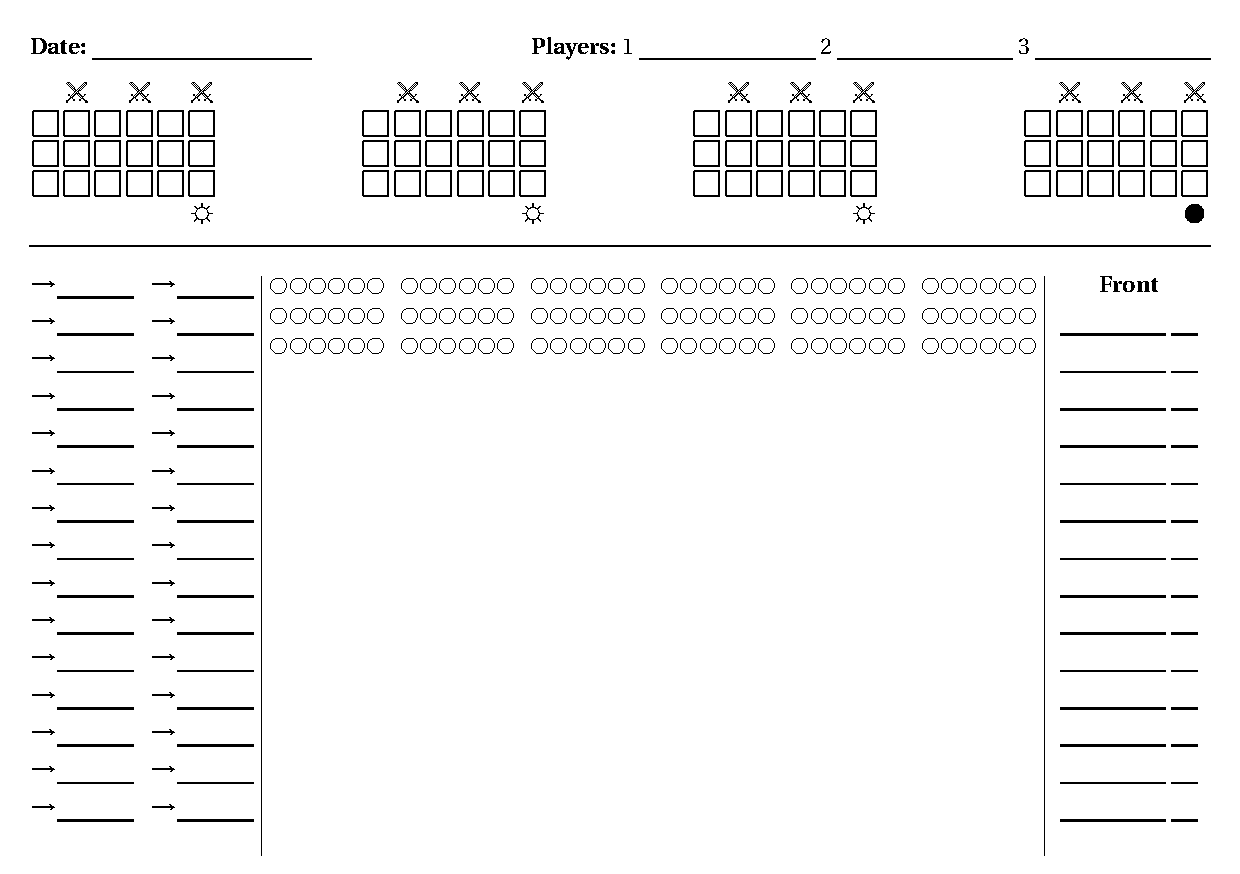
\includepdf[angle=90]{vendor/session-form.pdf}

\textbf{Room Numbers:}
%
The left-hand column is used to track the party's route through the dungeon;
this is mostly useful \emph{after} the session when it comes to restocking.
%
I only make ``restock rolls'' for rooms the party \emph{saw empty}, not for all
rooms that in fact \emph{are empty}.

\textbf{Marching Order:}
%
The right-hand column has the party's \emph{marching order} including who
carries what kind of \emph{light source} (L = lamp, T = torch, M = magic); I
encourage single-file simply because it means fewer PCs falling into bottomless
pits, but I am flexible if players \emph{insist} on walking next to each other
(I just put a line next to ``pairs'' on the far right).

\textbf{Random Notes:}
%
The middle column is for free-form notes of \emph{any} kind; I usually track
hit points of monsters there, but also reminders of treasures found and other
changes the party made to the dungeon.
%
There is also a \emph{round tracker} but I only use it when I have to, for
example because a monster they just killed will get up again or because a
character only has a few rounds left to live.
\by{phf}


\begin{multicols}{2}

\section{Dungeon: Zisterne der Auferstehung}

\subsection{Kurzfassung}

Lange Zeit war der Artemistempel, nördlich von Quastenholm,
verlassen. Nur die Zisterne wurde von den Menschen noch genutzt. Vor
drei Jahren bahnte sich Balto einen Weg aus den Tiefen unter dem Tempel
an die Oberfläche. Entflohen aus seiner Gefangenschaft, versucht er zu
verhindern das seine Unterdrücker jemals an die Oberfläche kommen. Dazu
hat er sich eine kleine Gefolgschaft aus Werratten um sich gescharrt. Aus
den Tiefen hat er auch eine Faustgroße gallertartige Masse mitgebracht
und diese im, mit Wasser gefüllten, Zisternebecken ausgesetzt um ihre
Entwicklung zu beobachten.

Vor zwei Jahren trafen Alwin, der die vergrabene Siedlung nach
wertvollem absuchte, und Balto eine Abmachung. Alwin hält andere ab
in die vergrabene Siedlung zu gehen und Balto übergibt ihm monatlich
Schätze, die er dort gefunden hat. Die Abmachung konnte nicht lange von
Alwin gehalten werden, da nach 3 Monaten bereits Echsenmenschen nach
etwas in der Siedlung suchten. Also traf Balto mit den Echsenmenschen
eine Abmachung und überließ ihnen die Siedlung wenn sie andere davon
abhalten unter die Zisterne zu kommen.

Alwin hat durch Zufall herausgefunden das die Gallertmasse in der Zisterne
lange verstorbene Menschen wieder zurückbringen kann und nutz dies aus um
einen Kult um die Zisterne zu erschaffen. Durch einen weiteren Zufall ist
eine Werratte in seine Bann geraten, mit der er sich weitere Werratten
schafft um Balto von dort unten vertreiben zu können damit er selber
wieder nach den Schätzen suchen zu kann. Alwin verfolgt nur dieses Ziel,
und erkennt nicht die anderen Möglichkeiten die sich ihm bieten.

\subsection{Gerüchte}

\begin{tabularx}{\columnwidth}{cZ}
1 & Das Trinkwasser in und um Quastenholm ist versalzen. (wahr) \\
2 & Echsenmenschen versuchen Quastenholm zu übernehmen. (falsch) \\
3 & Knecht … hat in Bauer Bertrams Jauchegrube Gold im Wert eines 
    Jahreslohns gefunden (wahr, Eigang zu Ebene 2) \\
4 & Längst Verstorbene werden hier von den Toten zurückgebracht.
    Dafür braucht es nichts weiter als die Erinnerung an die Person. 
    (falsch, es werden Kopien, Gallertmenschen, aus den Erinnerungen 
    durch das Wesen in der Zisterne erschaffen). \\
\end{tabularx}

\subsection{Gallertmenschen}

\begin{tabbing}
Anzahl: 1\\
Gesinnung: siehe Beschreibung\\
Bewegung: 12'' [siehe Beschreibung]\\
Rüstungsklasse: 7 [12]\\
Trefferwürfel: 4\\
Angriffe: 1\\
Schaden: 2W6\\
Rettungswurf: K4\\
Moral: 6/12 [siehe Beschreibung]\\
Hortklasse: keine\\
\end{tabbing}

Sie entsprechen den wahren als auch falschen Erinnerungen der Personen die
die gallertartige Masse im Zisternenbecken berühren und überleben. Ihr
Körper besteht aus einer gallertartigen Masse, nur deren äußeres
Erscheinungsbild entspricht den Erinnerungen. Wird die Person, aus
dessen Errinerungen sie geschaffen wurde, attakiert oder getötet,
werden die Gallertmenschen wütend und kämpfen bis zum Ende.

Immun gegen Gift, Verzauberung, Lähmung und Versteinerung.

\subsection{Raumbeschreibungen}

Räume 1 - 7 haben gemauerte Wände und Bodenplatten. Alle anderen
``Räume´´ wurden von den Werratten mit den Händen gegraben und bestehen
aus Erde und Steinen. Die Wände und Böden sind weder glatt noch eben.
Die Werratten in menschlicher Form haben lange, dünne Schnautzbärte
(Männer und Frauen).

Nördlich von Quastenholm steht ein alter, nicht mehr genutzter
Artemis Tempel. Über die Dachrinnen des Tempels wird Regenwasser
in das Zisternenbecken geleitet. In 3~m Höhe sind 0,5~m x 0,5~m große
Fensteröffung im Abstand von 3~m angeordnet um den Innenräumen Licht zu
spenden. Die Tür des Tempels liegt vor dem Eingang. Südlich des Tempels
steht ein Brunnen der direkt in das Zisternenbecken (Raum 4) führt.

\bigmap{img/Zisterne1und0.png}

\subsection{Ebene 0}

\subsubsection{1 - Zeremonienraum:} Jeweils an der Nord- und an der Südwand stehen drei
Statuen die Artemis in einer Jagdpose zeigen. In der Mitte des Raumes
liegen aufgehäufte Holz- und Schuttreste. Die Tür zum Nachbarraum ist
angelehnt. Unter der südwestlichten Statue ein durchbruch zu G1. In
der Nähe der dieser Statue befinden Schleifspuren auf den Bodenplatten.

\subsubsection{2 - Hinterraum:} Entlang der Wände haben Ratten aus Unrat und Holzresten
ihre Nester gebaut. In dem Raum befinden 32 Ratten (6 Rudel), die sich
aber nur aggressiv Verhalten wenn man sich ihnen oder ihren Nestern
nähert. Im Nest am südöstlichsten Punkt im Raum steckt ein mit
Feueroplaen besetzter goldener Gürtel(500~GM). Eine Wendeltreppe führt
nach unten in den Keller.  

\textbf{Rattenrudel} TW~1~TP RK~9 1W6 + Krankheit NM
BW~6'' (schwimmend 3'') ML~5 EP~10 

Krankheit: 1 in 20 Chance auf Infektion. Rettungswurf
gegen Gift. 1 in 4 Chance Tod in 1W6 Tagen, ansonsten ist das Ziel krank
und bettlägerig für einen Monat.

\subsection{Ebene 1}

\subsubsection{3 - Keller:} Die Wendeltreppe führt hinauf in den Hinterraum (Ebene
0). Südlich der Wendeltreppe lauert eine riesige Schwarze Witwe an
der 3 Meter hohen Decke.  In der Südostecke des Raumes hängt ein
Spinnenetz. Darunter liegen meschliche Knochen und 65~GM. An der östlichen
Wand ist ein Durchbruch zu Raum 12.  

\textbf{Riesige Schwarze Witwe} TW~3* RK~6 2w6 + Gift K2 BW~6'' (12''
im Netz) ML~8 EP~300 
Gift: tötet Opfer innerhalb einer Phase (Rettungswurf Gift)

\subsubsection{4 - Zisterne:} Ein Steg führt um das Zisternenbecken. An allen vier
Wänden hängen große Wandteppiche. Hinter dem westlichen befindet sich
der Zugang zu Raum 7. Vier schmucklose Säulen stützen die Decke. Ein
Wanddurchbruch verbindet die Zisterne mit Raum 9.  

Das Zisternenbecken ist
gefüllt mit einer gallertartigen Masse die sich von Wasser ernähert. Sie
ist durchsichtig. Wer sie berührt muss einen Rettungswurf gegen Tod
durchführen. Bei einem Fehlschlag stirbt der Berührende sofort an
einem Herzstillstand. Die Masse entzieht dem Opfer über 1W6 Tage das
Körperwasser und entsorgt den wasserlosen Rest im Loch in der Mitte
des Zisternenbeckens. Bei Erfolg erschafft die Masse ein Ebenbild
(Gallertmensch) der am meisten vermissten Person innerhalb der nächsten
2W6 Tage. 

Der Gallertmensch entspricht sowohl den wahren als auch falschen
Erinnerungen des Berührenden.  Die Masse selber erleidet keinen Schaden
durch Waffen oder Magie und kann auch nicht vergiftet, versteinert oder
verzaubert werden. Sie möchte immer weiter wachsen indem sie immer
mehr Wasser aufnimmt. Wasser nähert sie sich langsam, folgt aber der
verlockung großer Wasseransammlungen.

\subsubsection{5 - Predigtenraum:} 2 in 6 Chance das Alwin (s.u., Raum 6)
eine Predigt abhält. Zuhörer
der Predigt bestehen aus 1W6 normale Menschen mit 1W4-1 Gallertmenschen
sowie 1W4 Werratten (in Menschenform) mit 1W4-2 Gallertmenschen. 

Wird von
dem Steinpodest an der Nordwand gesprochen muss jeder den Anweisungen
für 1W6 Tage folgen, wenn ein Rettungswurf gegen Zaubersprüche nicht
geschafft wurde. 

Der Wandteppich im Süden Raumes verdeckt den Zugang
zu Raum 7. Vor dem Podest stehen 3 alte, 8~m lange Holzbänke. Die
Geheimtür im Nordwesten des Raumes kann durch das leichtes drücken
geöffnet werden, wenn man sie entdeckt hat.  

\textbf{Werratten} TW 3* RK 7 (9
in menschlicher Form) 1W6~(Biss) oder 1W6~(Waffe) K3 BW~12'' ML~8 EP~350
[4 in 6 Chance auf erfolgreichen Hinterhalt] 

\textbf{Normale Menschen} TW 1/2 RK 9 1W6~(Knüppel) NM BW~12'' ML~6 EP~50

\textbf{Gallertmenschen} TW~4 RK 7 2W6 K4 BW~12'' ML~6/12 EP~400

\subsubsection{6 - Bibliothek:} In den größtenteils leerstehenden Regalen befinden
10 Tontafeln (Spruchrollen)[5 x Schutzrolle vor Bösem, Schild,
Unsichtbarkeit, Klopfen, Feuerball Wachstum von Pflanzen]. In der
der nordöstlichen Ecke befindet sich ein Schreibplatz auf dem ein
Schreibgriffel liegt. In der nordwestlichen Ecke steht eine Statue der
Artemis, hinter der ein Geheimraum mit einer, nach obenführenden, Leiter
ist. Vor der Statue befinden sich Kratzspuren auf den Bodenplatten. 1 in
6 Chance das die Statue nicht vor der Öffnung zum Geheimraum steht. 1
in 6 Chance das sich Alwin in dem Raum befindet.  

\textbf{Alwin [Medium]} TW~1 RK~9
1W6 (Dolch) oder Zauberspruch M1 BW~12'' ML~7 EP~100 [1 x Schutz vor Bösem]
 

\subsubsection{7 - Geheimtunnel:} In der Ecke in einer verschlossenen Truhe befinden sich
400~GM. Dahinter gegen die Wand gelehnt steht Borstenschreck. Wandteppiche
grenzen den Geheimtunnel von Raum 4 und 5 ab. Drei Meter oberhalb des nördlichen
Ausgangs befindet sich ein Loch in der Wand (führt zu Gang G1).
Borstenschreck: magischer Speer +2 mit Elfenbeinschaft (Szenen einer
Wildschweinjagd sind auf dem Schaft dargestellt)

\subsubsection{8 - Höhle mit Falltür:} Dieser Bereich ist leer. Am südlichen Ausgang
befindet eine, mit lockerer Erde verdeckte, Falltür (Scharniere am
südlichen Ende). Wer die Falltür betritt fällt 3~m tief in ein 4~m
tiefes Wasserbecken. Schwere Rüstungen und hohe Traglast verhindern das
Schwimmen und ziehen zum Grund.  Die Falltür wird von den Werratten
regelmäßig kontrolliert und wieder geschlossen und verdeckt. Durch
den Durchgang in der Wand kann ein Halbling kriechen (oder Riesenratten).

\subsubsection{9 - Höhle mit Riesenschlagfalle:} An der westlichen Wand befindet sich
eine Anhäufung von Münzen (900~KM, 400~SM). Die Erde der Wand hinter dem
Haufen ist sehr glatt (durch den Bügel der Schlagfalle geglättet). Die
Riesenschlagfalle ist in den Boden eingelassen. Der Eisenbügel ist
sichtbar und nicht versteckt. Die Falle wird ausgelöst sobald Münzen
von dem Haufen genommen werden. Ein erfolgreicher Rettungswurf gegen
Odem verhindert das der Abenteurer vom Bügel der Schlagfalle erschlagen
(sofortiger Tod) wird. Im Norden ist die Wand zu Raum 4 durchbrochen.

\subsubsection{10 - Schlafplatz von Alwins Getreuen:} In diesem Bereich wohnen alle die
Alwin treu ergeben sind, egal ob aus freien Stücken oder beeinflusst
durch die Magie des Podestes aus Raum 5. Es sind 1W6 Werratten (in
menschlicher Form) und 1W2 normale Menschen anwesend. Jeder anwesende
Mensch und jeden anwesende Werratte ist mit seinem Gallertmenschen dort.
Ein Paar bewacht zwei Diamanten (500~GM und 300~GM wert).  

\textbf{Werratten} TW~3* RK~7 (9 in menschlicher Form) 1W6~(Biss) oder 1W6~(Waffe)
K3 BW~12'' ML~8 EP~350 [4 in 6 Chance auf erfolgreichen Hinterhalt] 

\textbf{Normale Menschen} TW~1/2 RK~9 1W6~(Knüppel) NM BW~12'' ML~6 EP~50 

\textbf{Gallertmenschen} TW~4 RK~7 2W6 K4 BW~12'' ML~6/12 EP~400

\subsubsection{11 - Schlafplatz der autonomen Werratten:} Hier ruhen 1W4 Werratten in
Riesenrattenform. Sie bewachen die Schätze der Werratten die weder
mit Alwin noch mit Balto zusammenarbeiten. Die Schätze sind in einem
Geheimraum, der durch einen Tunnel erreicht werden kann. Durch den Tunnel
passen Riesenratten, ein Halbling könnte ebenfalls durchkriechen. Eine
Diamanten besetzte, goldene Schwertlilienbrosche (500~GM) und ein
magisches Bronzekurzschwert sind hier versteckt.  

\textbf{Werratten} TW~3* RK~7 1W6(Biss) oder 1W6(Waffe) K3 BW~12'' ML~8 EP~350 [4 in 6 Chance auf
erfolgreichen Hinterhalt] Magisches Bronzekurzschwert: +1 Kurzschwert,
gegen Lykanthropen +2

\subsubsection{12 - Schatzhöhle:} In den Wände befinden sich auf 1~m Höhe insgesamt 40
kleine Öffnungen, die alle 0,5~m in die Wand gehen. In die Öffnungen
passt gerade so ein Arm hinein. Alle enthalten 1W10~EM und 1W20~GM. Ein
Abenteurer kann 10 Öffnungen in einer Phase leeren.

\subsubsection{G1 - Geheimer Kriechgang:} Der Gang ist so niedrig (60~cm) das selbst
Halblinge und Zwerge nicht aufrecht stehen können. Um in Raum 1 zu
gelangen darf die Artemisstatue den Durchgang nicht verdecken. Zu Raum
6 führt eine Leiter nach unten. Die Öffnung zu Raum 7 ist 3~m oberhalb
des Boden des Raumes.

\subsubsection{G2 - Baltos alte Experimentierhöhle:} Die Decke ist 1,5~m hoch. 4
Skeletthunde bewachen, mit Gelbschimmel überzogene, Rubine (50~GM, 18~GM,
113~GM, 76~GM, 89~GM, 5~GM, 29~GM, 47~GM, 112~GM, 63~GM) sowie wie einen ebenfalls
mit Gelbschimmel überzogenen Zauberstab der Lähmung [2 Ladungen]. Die
Gegenstände liegen an der westlichen Wand. Die Skeletthunde verlassen
den Raum nur wenn die Gegenstände gestohlen werden oder sie angegriffen
werden.  

\textbf{Skeletthunde} TW~1 RK~7  1W6 K1 BW~12'' ML~12 EP~100 

\textbf{Gelbschimmel} TW~2 RK~- 1W6 + Ersticken K2 BW~0'' ML~12 EP~200 [Schaden nur durch Feuer (1W4)]

Ersticken: Rettungswurf gegen Tod, Fehlschlag Tod in 6 Runden

\by{olupo}




\end{multicols}

\section{Impressum}

\textbf{Autoren}:

alex -- Alex Schröder, @kensanata@tabletop.social

lkh -- Laurens Kils-Hütten, @wandererbill@tabletop.social

olupo -- Olupo, @Olupo@rollenspiel.social

phf -- Peter H. Fröhlich, @phf@tabletop.social

ff -- Sören Kohlmeyer, @fastfox@pnpde.social

\textit{Grenzland} wird editiert und
herausgegeben von Laurens Kils-Hütten,
a.k.a. Wanderer Bill
email: wandererbill@betola.de, web: https://betola.de/wandererbill

Alle Inhalte stehen unter der Creative Commons Lizenz
Namensnennung -- Weitergabe unter gleichen Bedingungen 4.0 International (CC BY-SA 4.0)\\
http://creativecommons.org/licenses/by-sa/4.0/

Außerdem ist \textit{Grenzland} ein Open Source Projekt. Du
findest die Quelldateien unter
https://github.com/lskh/Grenzland-Zine
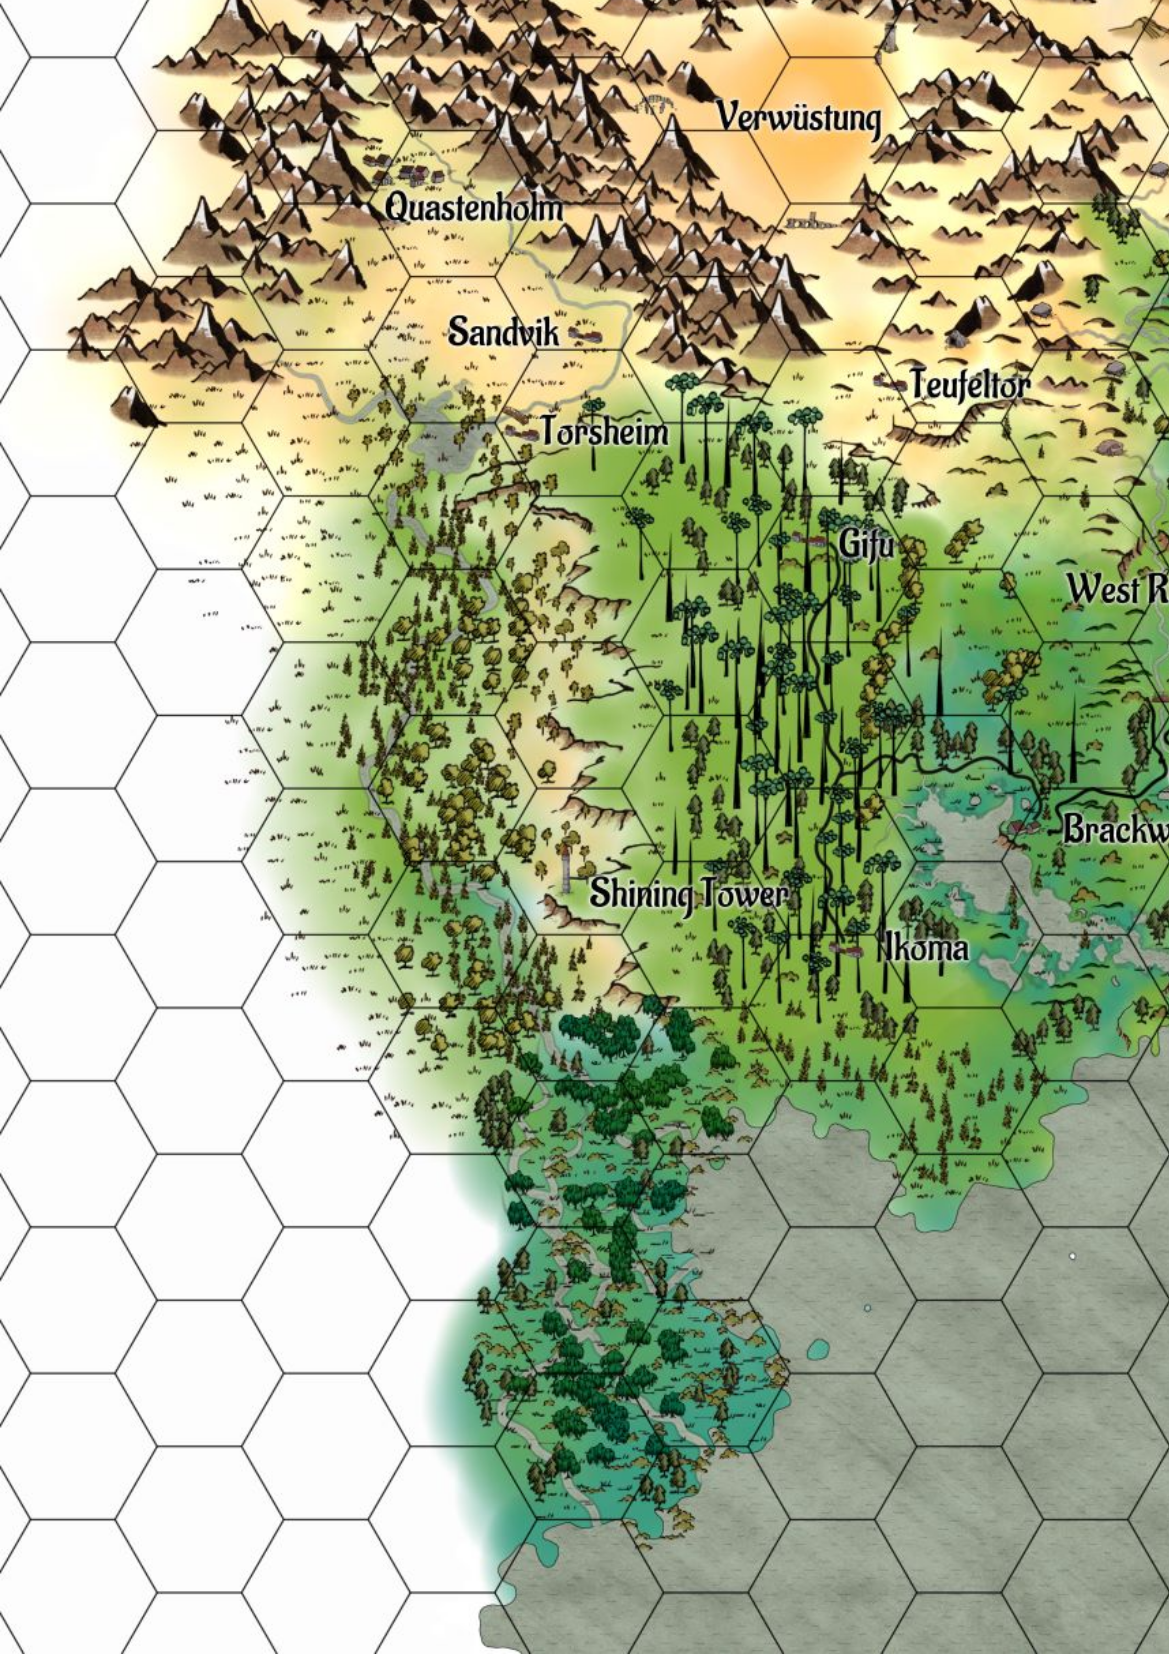
\includepdf{Backcover.pdf}
\end{document}
